\subsection{Zielbestimmung}

Heutzutage günstig Lego-Sets zu erwerben kann auf mehreren Ebenen ein wohlüberlegtes Unterfangen sein. Welche der Lego-Händler bieten die Sets günstig an? Ist es günstiger sich die Einzelteile des Sets einzeln zu bestellen? Was ist wenn bestimmte Einzelteile nicht mehr verfügbar sind? \newline
Das Ziel des Projekts ist genau diese Fragestellungen, durch die Entwicklung eines Tools zur Ermittlung der günstigsten Anbieter, zu beantworten. Das Tool soll dabei auch in der Lage sein, abzuwägen, ob es günstiger ist, das Set oder Einzelteile zu kaufen und zu kombinieren.

\subsubsection{Musskriterien}
Interne Teileverwaltung durch das Pflegen einer Datenbank über die Einzelteile. \newline 
Die PDF-Bauanleitungen der Lego-Sets sollen mit OCR auslesbar sein. \newline
Ein Crawler bezieht die Preise der unterschiedlichen Händler. \newline
Ein Preisvergleich unter den Händlern, im Bezug auf Kauf eines Sets oder die jeweiligen Einzelteile, findet statt. \newline
Darstellung des Tools als graphische Oberfläche. (Startseite, Benuterverwaltung, Preisvergleich, Warenkorb) \newline
Es soll möglich sein Benutzeraccounts anzulegen und diese verwalten zu können. \newline
Drei feste Händler sollen beim Vergleich berücksichtigt werden. \newline
Der Warenkorb soll automatisch befüllt werden. \newline
Auf nicht verfügbare Einzelteile sollte hinreichend hingewiesen werden. \newline
Die Lieferkosten sollen beim Preisvergleich berücksichtigt werden. \newline 
Bei der Ausgabe des Vergleichs soll eine Verlinkung zum Produkt, sowie eine Liste der Bauteile, angezeigt werden. \newline
\subsubsection{Kannkriterien}
Test
\subsubsection{Wunschkriterien}
Einzelteile die besonders selten/teuer sollten gesondert aufgelistet werden \newline
Filterfunktion um zum Beispiel Figuren rauszufiltern \newline
Mehr Händler berücksichtigen \newline
Grafische Weboberfläche responsive designen \newline
Sticker berücksichtigen \newline
Benutzeraccount mit Wunschliste? (Historie) \newline
Eigene Bauanleitung auslesen lassen \newline
Aktuelle Angebote hervorheben \newline
Dashboard: Statistiken zum Suchverhalten unserer Benutzer / Wie erfolgreich war unser Programm? \newline

\subsubsection{Abgrenzungskriterien}
Unser Produkt wird keine Verkaufsplattform haben  \newline
Keine Bevorzugung von Händlern \newline
Wir berücksichtigen keine nicht offiziellen Klemmbausteine \newline
Website ist nur für deutschsprachige Benutzer \newline
Alte Sets ohne Stückliste in der Anleitung können nicht berücksichtigt werden (2006) \newline

\subsection{Produkteinsatz}
 Das Produkt soll Benutzer bei Kaufentscheidung unterstützen, außerdem unterstützt es die Benutzer Sets zu bauen die aus irgendwelchen Gründen nicht mehr verfügbar sind.\newline
Das Tool ist für Lego-Enthusiasten und Sammler gedacht, die nach dem günstigsten Angebot suchen. Das Tool kann auch von Einzelpersonen oder Unternehmen genutzt werden, die große Mengen an Lego-Sets kaufen möchten. \newline

\subsection{Produktfunktionen}

\subsubsection{Produktfunktion Benutzer Sicht} \newline \newline
/F10/\newline
Geschäftsprozess: Über eine Suchmaske können Lego Setnummern eingeben\newline
Vorbedingung: User befindet auf der Website des LegoGCT\newline
Nachbedingung: Nach der Eingabe wird die Datenbank auf die Existenz des Lego Sets geprüft\newline
Fehlerfall: Die Eingegebene Setnummer stimmt nicht mit einer in der Datenbank vorhanden Setnummer überein. Oder Syntaxfehler führt zur falschen Eingabe\newline
Anwender: Akteur im Kontext der Webapplikation\newline
Beschreibung: Über die Suchfunktion kann der Benutzer eine Setnummer eingeben.\newline\newline
/F20/\newline
Geschäftsprozess: Anzeigen der Historie\newline
Vorbedingung: Benutzer sollte auf der Webplattform angemeldet sein\newline
Nachbedingung: Benutzer kann sich seine persönliche Historie anzeigen lassen\newline
Fehlerfall: Benutzer hat bisher noch keinen Suchvorgang gestartet\newline
Anwender: Akteur im Kontext der Webapplikation\newline
Beschreibung: Für Angemeldete Nutzer steht die Historie vergangener Suchen zur Verfügung. Diese unterstützt den Benutzer bereits gesuchte Sets wiederzufinden.\newline\newline
/F30/\newline
Geschäftsprozess: Registrierung auf der Webplattform\newline
Vorbedingung: User befindet auf der Website des LegoGCT und hat den Registrieren Button gedrückt\newline
Nachbedingung: User konnte sich Erfolgreich registrieren lassen sein Benutzer Account wurde in einer Datenbank abgelegt\newline
Fehlerfall: E-Mail ist bereits vergeben, Datenbank ist nicht ansprechbar, Passwortsicherheit zu gering\newline
Anwender: Akteur im Kontext der Webapplikation\newline
Beschreibung: Um die vollen Funktionsumfang der Webapplikation zu nutzen. Muss der Benutzer eine Registrierung durchführen.\newline\newline
/F40/\newline
Geschäftsprozess: Anmeldung auf der Webplattform\newline
Vorbedingung: Benutzer befindet auf der Website des LegoGCT und ist ein Registrierter Nutzer\newline
Nachbedingung: Benutzer konnte sich erfolgreich an Webplattform anmelden\newline
Fehlerfall: Eine Anmeldung war nicht erfolgreich, weil Passwort und Benutzername nicht übereinstimmen oder der Benutzer noch keine Registrierung vorgenommen hat.\newline
Anwender: Akteur im Kontext der Webapplikation\newline
Beschreibung: Um die volle Funktion der Webapplikation nutzen zu können, kann sich der Benutzer an der Webplattform anmelden\newline\newline
/F50/\newline
Geschäftsprozess: Darstellung der Stücklisten\newline
Vorbedingung: Benutzer hat nach einer Setnummer gesucht, welche in der Datenbank vorhanden ist.\newline
Nachbedingung: Benutzer bekommt eine Stückliste mit Einzelteilen angezeigt \newline
Fehlerfall: Stückliste konnte nicht dargestellt werden, da zu viele Einzelteiler bei Händler nicht zur Verfügung stehen. \newline
Anwender: Akteur im Kontext der Webapplikation \newline
Beschreibung: Dem Benutzer wird eine Stückliste des Legosets ausgegeben nach dem der Benutzer gesucht hat. Die Stückliste enthält die Einzelteile mit folgenden Attributen Einzelteilnummer, Anzahl, Preis, URL \newline\newline
/F60/\newline
Geschäftsprozess: Minimieren der Stücklisten\newline
Vorbedingung: Benutzer bekommt eine Stückliste mit Einzelteilen angezeigt\newline
Nachbedingung: Benutzer bekommt nur noch den Endpreis angezeigt\newline
Fehlerfall: keinen\newline
Anwender: Akteur im Kontext der Webapplikation \newline
Beschreibung: Der Benutzer möchte eine übersichtlichere Anzeige haben und minimiert deshalb die Stückliste, um sich den Endpreis übersichtlicher darstellen zu lassen.\newline\newline
/F70/\newline
Geschäftsprozess: Anzeigen des Endpreises \newline
Vorbedingung: Benutzer \newline
\subsubsection{Produktfunktionen Backend}\newline
PDFs mit Crawler ansprechen können \newline
PDFs mittels OCR auslesen \newline
Einzelteile in Datenbank zwischenspeichern \newline
Informationen bei Händlern abfragen können \newline
Preisvergeich zwischen Sets und Einzelteilen \newline
Darstellung der Endergebnisse \newline

\subsection{Produktdaten}

\subsubsection{Bauteil}
Element-ID\newline
Name \newline

\subsubsection{Bauteil/Set-Preis}
Element-ID\newline
Preis\newline
Anbieter\newline
URL\newline

\subsubsection{Set}
Set-ID \newline
List: Element-ID \newline
Name \newline
Bool: Verfügbarkeit \newline
UVP \newline  \newline
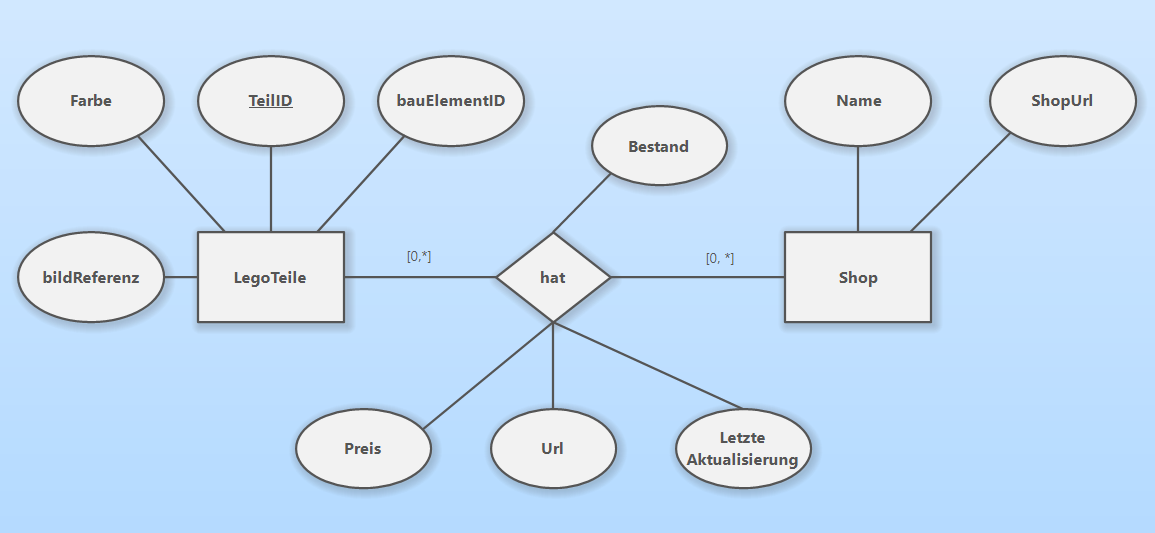
\includegraphics[width=8cm]{pictures/chen1.png} \newline  \newline
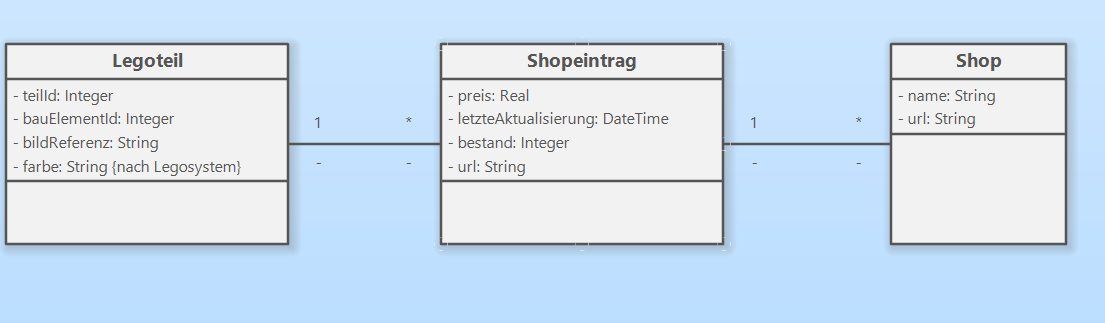
\includegraphics[width=8cm]{pictures/klassendiagramm2.png}  \newline  \newline
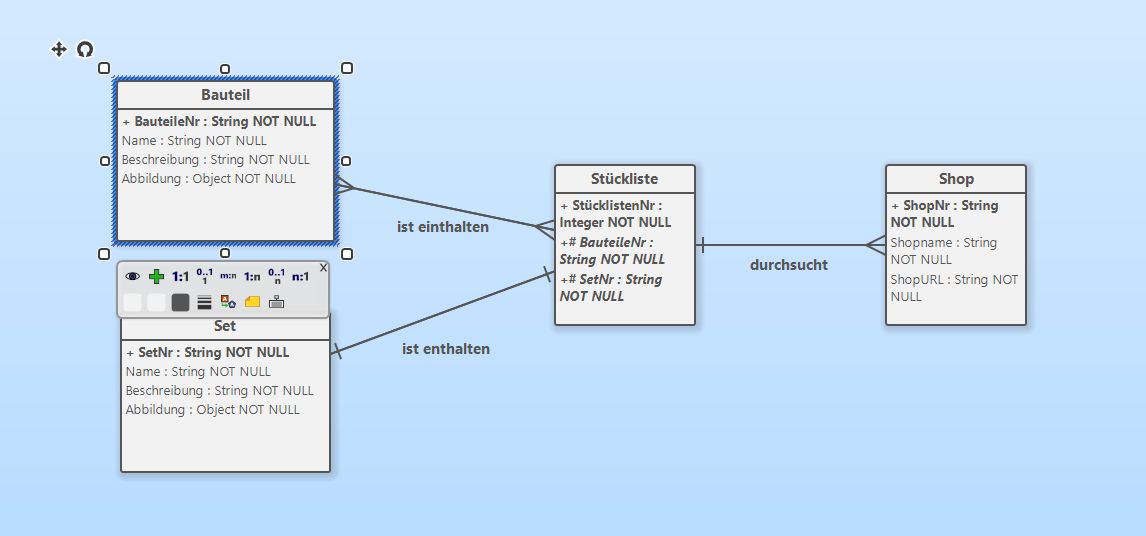
\includegraphics[width=8cm]{pictures/klassendiagramm.png} 

\subsection{Produktleistungen}
Bestandsdatenbank soll aufgebaut werden mit Informationen aus den Anleitunge \newline
Preise sollen bei der Suche gecrawlt werden \newline
Die verwendete Datenbank muss in der Lage sein große Datenmengen zu speichern und zu verarbeiten \newline
Der Crawler soll in der Lage sein schnell Preisdaten bei den Anbietern zu crawlen, außerdem soll ein Algorithmus regelmäßig die neuen Anleitungen erkennen und dem Parser übergeben \newline

\subsection{Qualitätsanforderungen}
Dokumentation der Änderungshistorie \newline
Programmcode auskommentieren \newline

\subsection{Benutzungsoberfläche}
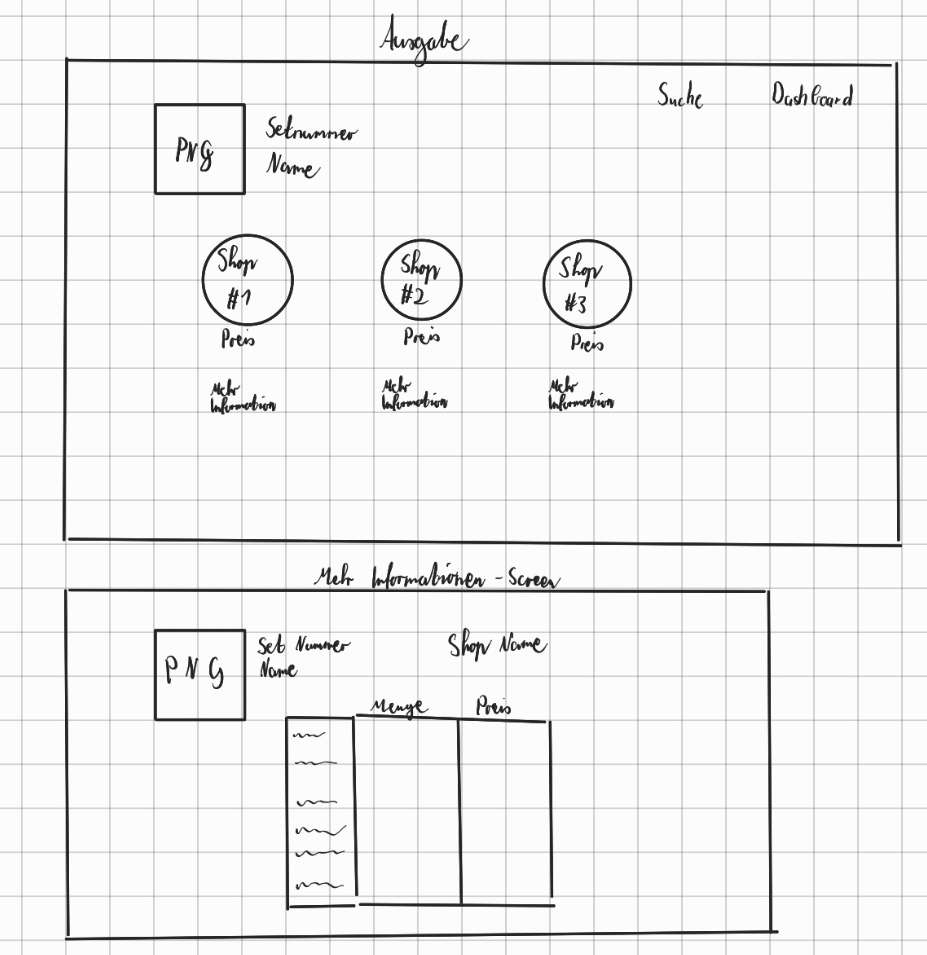
\includegraphics[width=8cm]{pictures/skizzeausgabe.jpg} \newline \newline
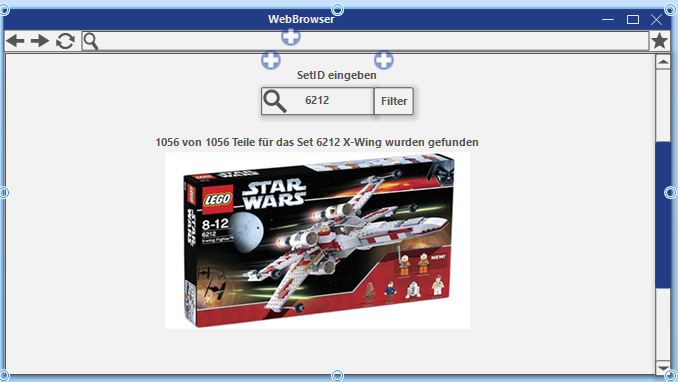
\includegraphics[width=8cm]{pictures/programmvorschau1.png}
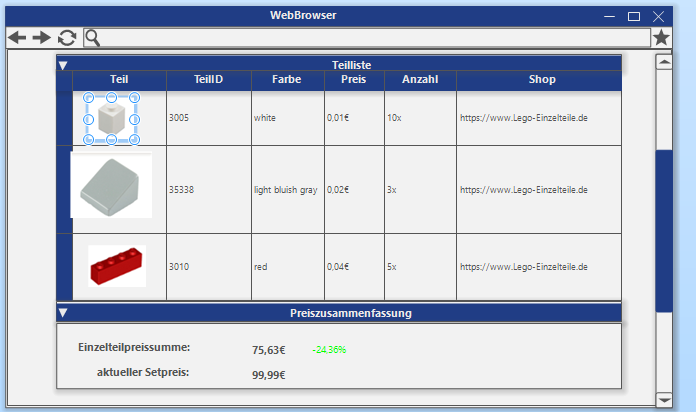
\includegraphics[width=8cm]{pictures/programmvorschau2.png} \newline \newline

\includegraphics[width=8cm]{pictures/programmvorschau3.png}

\subsection{Nichtfunktionale Anforderungen}
Barrierefreiheit \newline
Intuitives Design \newline
ISO Normen aus dem MCIW-Modul einhalten \newline
Revisionsinstanzen Scrum etablieren \newline
Websitendaten schützen die gecrawlt werden \newline

\subsection{Technische Produktumgebung}
Datenbank \newline
Crawler \newline
Webserver \newline
OCR \newline
Angular \newline
HTML \newline
CSS \newline
Python \newline
Tex \newline
Git \newline

\subsection{Gliederung in Teilprodukte}
Bauanleitung suchen \newline
Bauanleitung parsen \newline
Datenbank füllen \newline
Preisvergleich \newline
Ausgabe generierern \newline
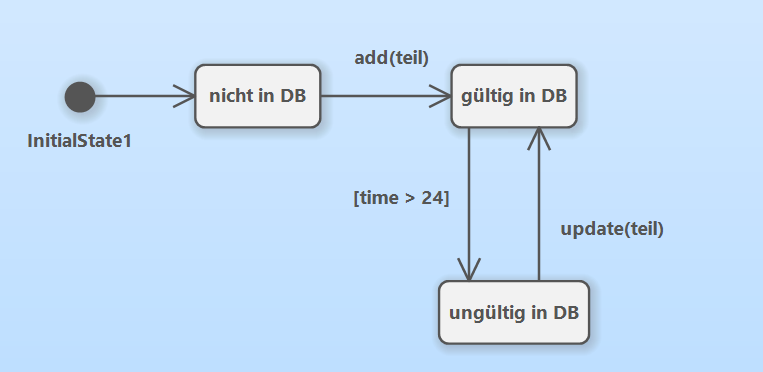
\includegraphics[width=8cm]{pictures/datenbankupdate.png} \newline  \newline
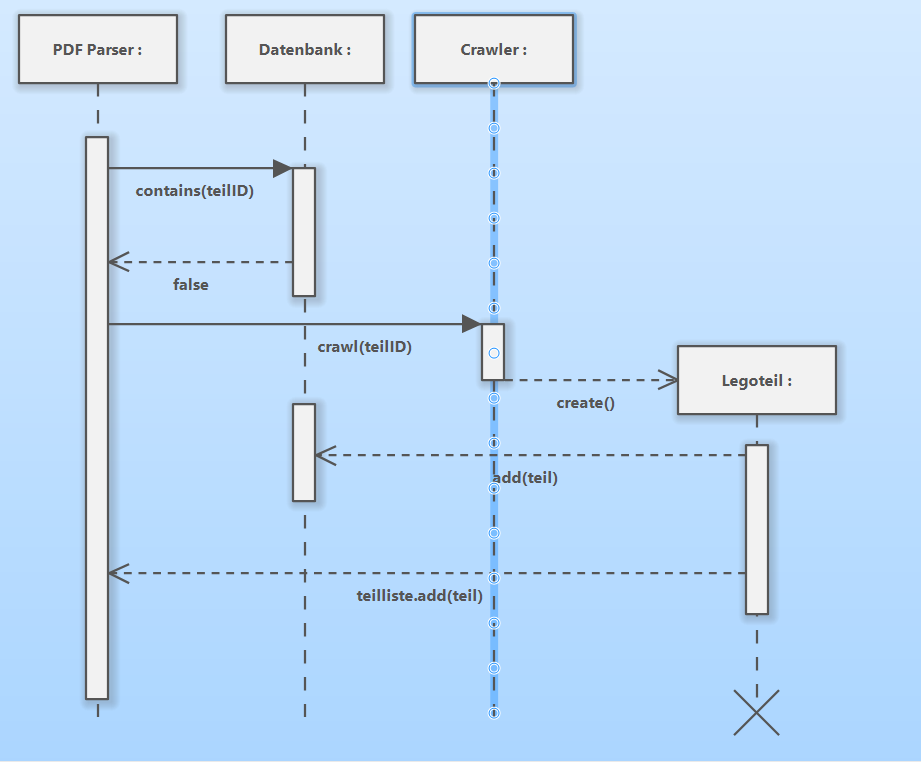
\includegraphics[width=8cm]{pictures/vorgaenge.png}


\subsection{Ergänzungen}
Aus rechtlichen Gründen sollen Anbieter vor dem Crawling angefragt werden \newline
Installationsanleitung und Handbuch sollen bereitgestellt werden \newline

\subsection{Globale Testfälle}
Set händisch recherchieren, um Soll-Wert für Unit-Test zu ermitteln und mit Algortihmusausgabe testen \newline
Set-ID mit Bauanleitung ohne Stückzahl \newline
Gülige Set-ID suchen \newline
Ungültige Set-ID suchen \newline
